\section{AFND Números binarios con terminación '01'}
	\subsection{Descripción del problema}
	Desarrollar un autómata finito no determinista, que acepte todas y sólo las cadenas formadas por ceros y unos que terminan en 01. Asimismo, imprimir la tabla de transiciones (historia) y que la entrada de cadenas sea de forma manual o automática, la cadena aleatoria debe de tener una longitud $n \mid 1  \leq n \leq 1000$. Y que contenga la opción de mostrar el siguiente diagrama.
	\begin{figure}[H]
		\begin{center}
			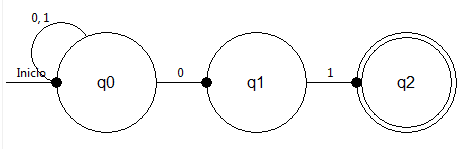
\includegraphics[width=12cm, height=4cm]{img/cero-uno.png}
			\caption{Diagrama de transiciones del autómata. \cite{LIBRO}}
			\label{fig:diagrama4}
		\end{center}
	\end{figure}
	\subsection{Código}
	El código fue realizado en Python 3.5.
	\\Archivo: main\_cero\_uno.py
	\begin{lstlisting}[language=Python]
	#main_cero_uno.py
	# -*- coding: utf-8 -*-
	from __future__ import print_function
	from automata_cero_uno import automata
	from diagrama_cero_uno import Diagrama
	import random
	
	separador = '*'*50
	
	def iniciar():
		continuar = True
		while continuar:
			opcion = imprimir_menu()
			if opcion == 1:
				entrada_consola()
			elif opcion == 2:
				ejecutar_random()
			elif opcion == 3:
				ver_diagrama()
			else:
				break # Sal del programa
			print('*' * 100)
			opcion = input("Reintentar s/n: ")
			if opcion.lower() != 's':
				continuar = False
		
		print('Saliendo del programa...')
	
	def imprimir_menu():
		print('\n\n%sMenu%s' % (separador, separador))
		print("""
		1.- Entrada en consola (Manual)
		2.- Aleatorio (Automatico)
		3.- Ver diagrama
		4.- Salir
		""")
		try:
			opcion = int(input("Selecciona una opcion valida: "))
			return opcion
		except Exception as e:
			print('Error ', e)
			return 0
	
	def entrada_consola():
		texto = input("Escribe el numero binario: ")
		automata(texto)
	
	
	def ejecutar_random():
		i = 0
		longitud_random = random.randint(1, 1000)
		numero_binario = ''
		while i < longitud_random:
			numero_binario += random.choice(['0', '1'])
			i += 1
		
		print("El numero aleatorio es: ", numero_binario)
		automata(numero_binario)
	
	def ver_diagrama():
		print('Mostrando diagrama del automata. Cierre la ventana para continuar')
		try:
			diagrama_ere = Diagrama()
			diagrama_ere.master.title('Diagrama del automata cero-uno')
			diagrama_ere.mainloop()
		except Exception as e:
			print("Error", e)
	
	
	iniciar()
	\end{lstlisting}
	Archivo: automata\_cero\_uno.py
	\begin{lstlisting}[language=Python]
	
	#automata_cero_uno.py
	# -*- coding: utf-8 -*-
	from __future__ import print_function
	
	def automata(text):
		array_tabla = []
		array = ['0']
		i = 0
		array_tabla.append(['0'])
		temporal_cero = []
		temporal_otro = []
		temporal = []
		for simbolo in text:
			array = array_tabla[i]
			for estado_evaluacion in array:
				if simbolo == '0' and estado_evaluacion == '0':
					temporal_cero = evaluar_estados(estado_evaluacion, simbolo)
				else:
					temporal_otro.append(evaluar_estados(estado_evaluacion, simbolo))
				
				if(len(temporal_cero) != 0):
					temporal.append(temporal_cero[0])
					temporal += temporal_otro[:]
					temporal.append(temporal_cero[1])
				else:
					temporal += temporal_cero[:]
					temporal += temporal_otro[:]
				array_tabla.append(temporal[:])
				temporal_cero = []
				temporal_otro = []
				temporal = []
				i += 1
		
		rellenar_tabla(array_tabla, text)
		letra = 0
		text +=' '
		print('')
		for linea in array_tabla:
			print(text[letra], end=' | ')
			for valor in linea:
				if(valor == '-1'):
					print("x", end=' ')
				else:
					print("q%s" %valor, end=' ')
				print()
				letra +=1
		
		if array_tabla[len(text)-1][len(array_tabla[len(text)-1])-1] == '2':
			print('El numero: %s es una cadena valida' % text)
		else:
			print('El numero: %s NO es una cadena valida' % text)
	
	def rellenar_tabla(array_tabla, text):
		longitud = len(text)
		ultima_fila = len(array_tabla[longitud])
		ceros = False
		if array_tabla[longitud][ultima_fila-1] == '2':
			ceros = True
		for fila in array_tabla:
			while True:
				if len(fila) >= ultima_fila:
					break
				if (len(fila)+1 >= ultima_fila) and ceros:
					fila.append('0')
				else:
					fila.append('-1')
	
	def evaluar_estados(estado, simbolo):
		if estado == '0':
			estado = estado_cero(simbolo)
		elif estado == '1':
			estado = estado_uno(simbolo)
		elif estado == '2':
			estado = estado_dos(simbolo)
		
		return estado
	
	def estado_cero(simbolo):
		if simbolo == '1':
			return '0'
		elif simbolo == '0':
			return ['0', '1']
	
	def estado_uno(simbolo):
		if simbolo == '1':
			return '2'
		else:
			return '-1'
	
	def estado_dos(simbolo):
		return '-1'
	
	\end{lstlisting}
		Archivo: diagrama\_cero\_uno.py
		\begin{lstlisting}[language=Python]
		#diagrama_cero_uno.py
		# -*- coding: utf-8 -*-
		from __future__ import print_function
		import tkinter as tk
		
		class Diagrama(tk.Frame):
			def __init__(self, master=None):
				super().__init__(master, background='white')
				self.pack(fill=tk.BOTH, expand=tk.YES)
				self.canvas = tk.Canvas(self, bg='white')
				self.canvas.pack(fill=tk.BOTH, expand=1)
				self.dibujarDiagrama()
				self.centrarVentana()
			
			def dibujarDiagrama(self):
				coordenadas = [55, 100, 155, 200]
				for x in range(3):
					self.escribirTexto(x, coordenadas)
					self.dibujarCirculo(coordenadas)
					self.dibujarFlecha([coordenadas[0]-50, 150, coordenadas[2]-100, 150])
					coordenadas[0] += 150
					coordenadas[2] += 150
				
				self.dibujarCirculo([coordenadas[0]-150+5, 105, coordenadas[2]-155, 195]) # circulo interior
				self.canvas.create_arc(30, 90, 90, 150, start=30, extent=235, style='arc')
				self.canvas.create_text(40, 85, text='0, 1')
			
			def escribirTexto(self, x, coordenadas):
				text = ''
				text_flecha =''
				if x == 0:
					text = 'q%s' % x
					text_flecha = 'Inicio'
				elif x == 1:
					text = 'q%s' % x
					text_flecha = '0'
				elif x == 2:
					text = 'q%s' % x
					text_flecha = '1'
				else:
					print('otro')
				
				self.canvas.create_text(coordenadas[0]+50, coordenadas[1]+50, font=('15'), text=text)
				self.canvas.create_text(coordenadas[0]-25, coordenadas[1]+40, text=text_flecha)
			
			def dibujarCirculo(self, arg):
				circulo = self.canvas.create_oval(arg)
			
			def dibujarFlecha(self, coordenadas):
				linea = self.canvas.create_line(coordenadas)
				self.canvas.create_oval(coordenadas[2]-5, coordenadas[1]-5, coordenadas[2]+5,coordenadas[1]+5, fill = 'black')
			
			def centrarVentana(self):
				ancho, altura = 500, 300
				ancho_pantalla = self.winfo_screenwidth()
				altura_pantalla = self.winfo_screenheight()
				posicion_x = (ancho_pantalla - ancho)/2
				posicion_y = (altura_pantalla - altura)/2
				self.master.geometry('%dx%d+%d+%d' % (ancho, altura, posicion_x, posicion_y))
		
		\end{lstlisting}
	\newpage
	\subsection{Pruebas}
	Pruebas de las opciones del menú.
	\\{\large Modo manual}
	\begin{figure}[H]
		\begin{center}
			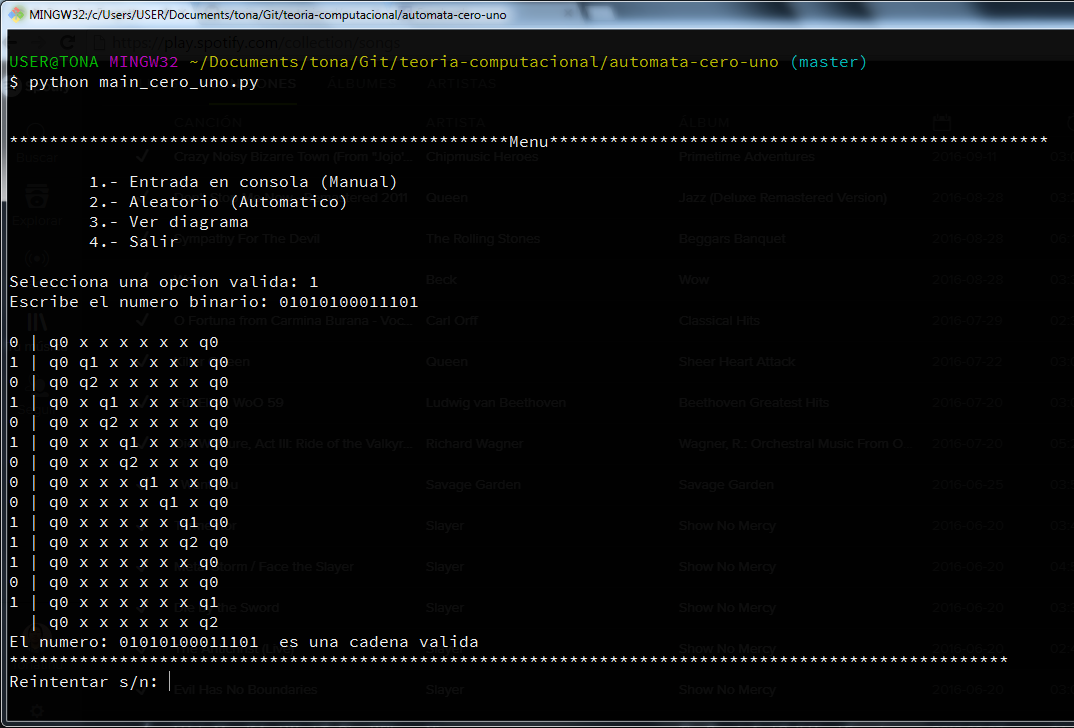
\includegraphics[width=\linewidth, height=8cm]{img/cero-uno-manual.png}
			\caption{Historia del autómata en una tabla}
			\label{fig:cero-uno1}
		\end{center}
	\end{figure}
	{\large Modo automático}
	\begin{figure}[H]
		\begin{center}
			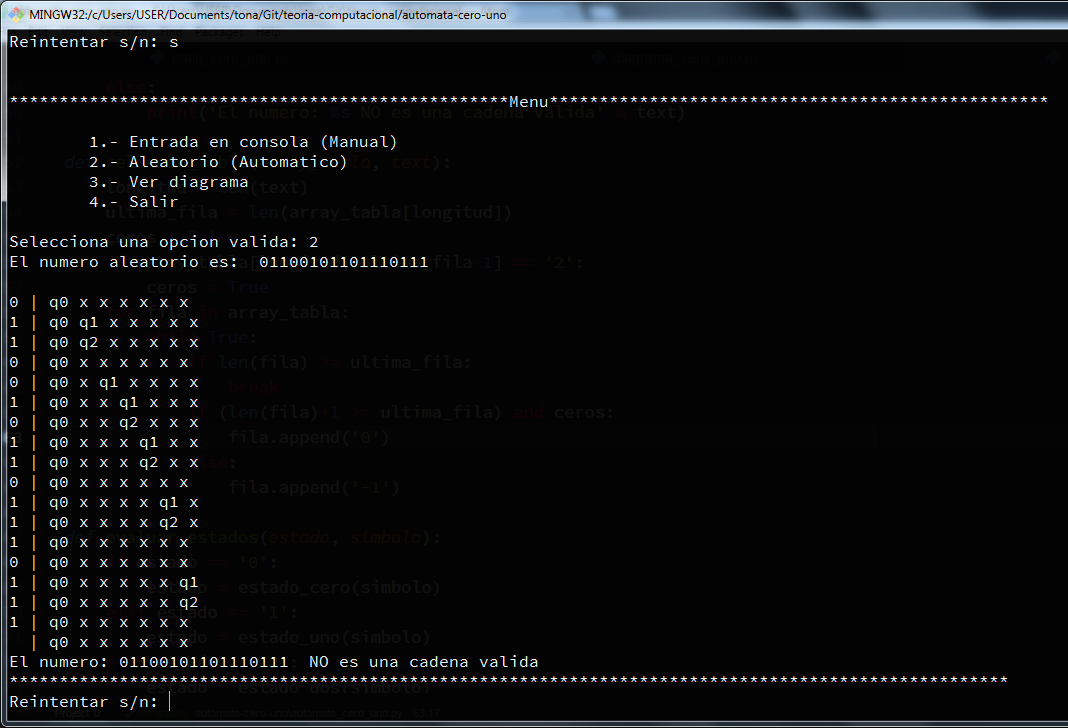
\includegraphics[width=\linewidth, height=8cm]{img/cero-uno-automatico.png}
			\caption{Historia del autómata en una tabla}
			\label{fig:cero-uno2}
		\end{center}
	\end{figure}
	{\large Diagrama}
	\begin{figure}[H]
		\begin{center}
			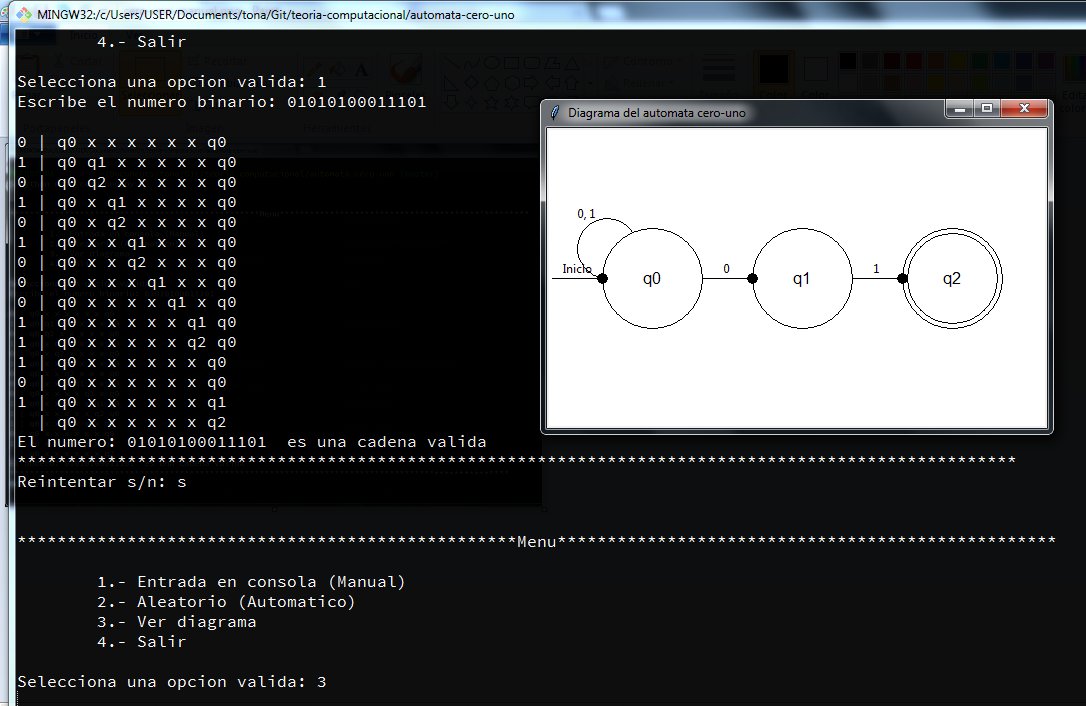
\includegraphics[width=\linewidth, height=10cm]{img/cero-uno-diagrama.png}
			\caption{Diagrama del autómata.}
			\label{fig:cero-uno3}
		\end{center}
	\end{figure}